\subsection{Bedienung des Editors}
Der Editor ist über den Text, Draw, Shape oder Image Button erreichbar. Genau wie im Reader erscheint ein Button Choose file. Je nachdem ob man auf Text, Draw, Shape oder Image geklickt hat, wird als erstes der Text-, Zeichen-, Geometrie- oder Bildeditor geöffnet. Hat man eine Datei geöffnet, so befindet sich der Reader ohne die Operationen zum Seiten Drehen ebenfalls im Editor, sowie seine Drag und Save Funktionalitäten. Bei Save kann man wie bei anderen Modulen einen benutzerdefinierten Dateinamen vergeben und das aktuelle PDF wird in den Downloads-Ordner runtergeladen. Alle input fields im Editor sind mit dem gültigen Wertebereich für Benutzereingaben als Information Min: Max: versehen. 

\subsubsection{Textbearbeitung}
Hat man den Texteditor aufgerufen, so präsentiert sich einem der Editor in folgenden Abbildungen \ref{fig:texteditor} und \ref{fig:texteditor2}.

\begin{figure}[!htbp]
	\centering
	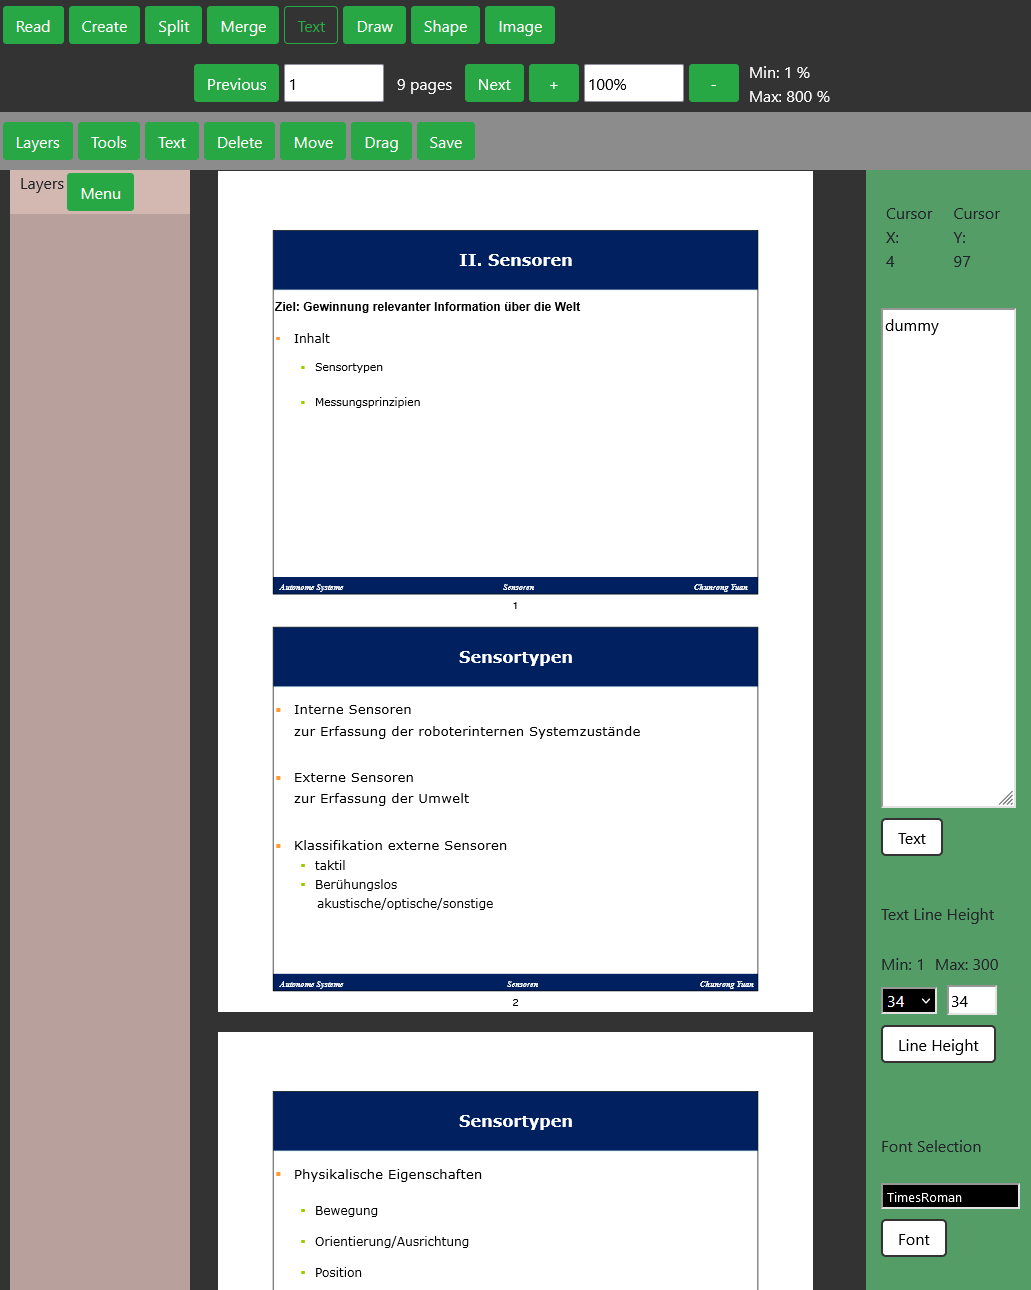
\includegraphics[width=1\textwidth]{"images/texteditor.png"}
	\caption{Startseite des Texteditors der PDF Web App}
	\label{fig:texteditor}
\end{figure}

\begin{figure}[!htbp]
	\centering
	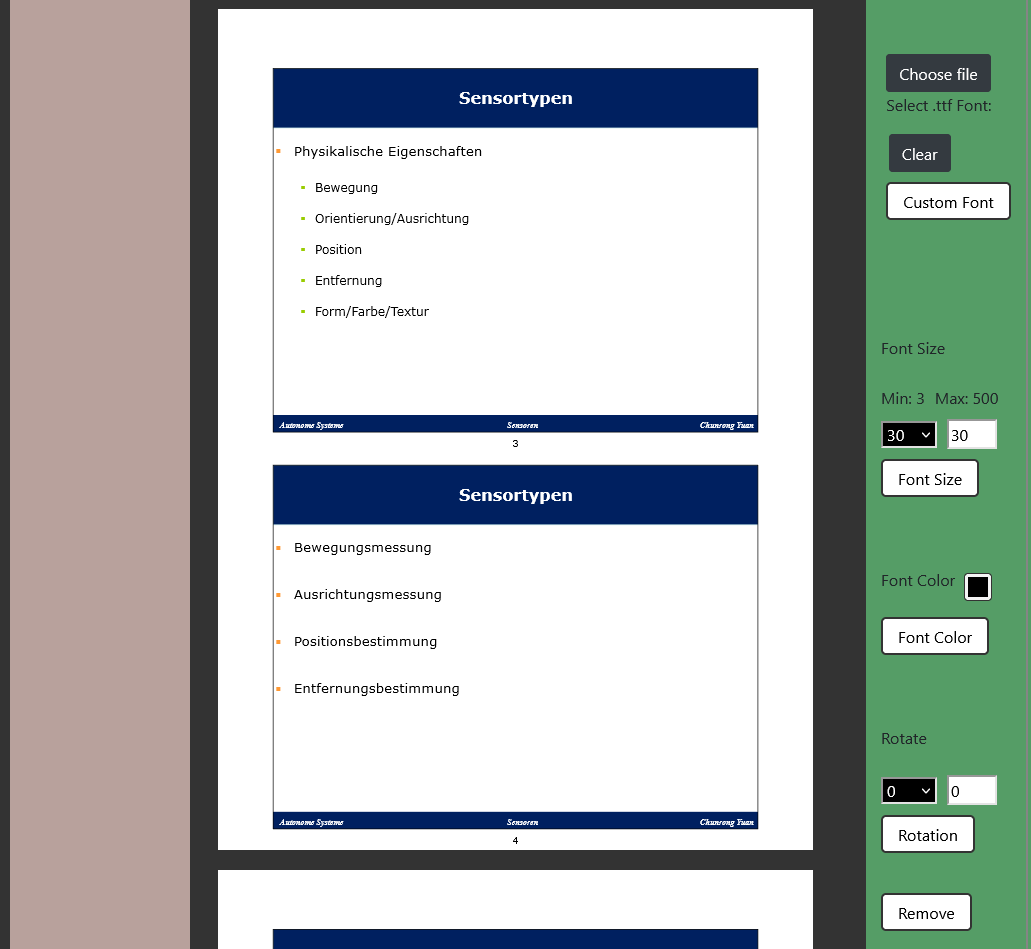
\includegraphics[width=1\textwidth]{"images/texteditor2.png"}
	\caption{Mehr Tools der Startseite des Texteditors der PDF Web App}
	\label{fig:texteditor2}
\end{figure}

Mit dem Button Text in der grauen Leiste und nachfolgendem Klick aufs geöffnete Dokument kann man einen Text hinzufügen mit dem Platzhaltertext dummy. Unter dem Text erscheint eine dunkelrote control box, auf die man alle Operationen in der grauen Leiste und dem Tools Seitenmenü im Box Mode anwenden kann. Der Box Mode ist standardmäßig eingestellt. Alle Operationen im rechten Tools Seitenmenü beziehen sich jeweils auf das aktuelle Editor Element und sind nur auf diesem anwendbar. Ich werde zunächst alle Operationen im Box Mode beschreiben und später auf den Layer Mode eingehen. Man kann mehrere Texte ohne erneut Text drücken zu müssen dem PDF Dokument hinzufügen. Für jedes neu hinzugefügte Textelement wird eine Ebene mit einem  Element spezifischen Standardnamen erstellt, was im linken rosa Ebenenmenü zu sehen ist. Mit dem Delete Button und nachfolgendem Klick in eine oder mehrere control boxen im Box Mode können Texte wieder gelöscht werden. Move verschiebt einzelne Texte durch mit der Maus gedrückte control box. Wenn die Maus losgelassen, nachdem die control box verschoben wurde, springt der Text an die verschobene Stelle. Ganz oben im grünen Tools Seitenmenü werden dem Betrachter die x- und y-Koordinaten der Maus auf der PDF Seite angezeigt, wenn die Maus über eine Seite bewegt wird. Darunter kann man in der textarea den Text editieren. Es werden auch Zeilenumbrüche berücksichtigt. Nachdem man den dummy Text überschrieben hat, einem Klick auf den weißen Text Button und ein oder mehrere Klicks in control boxen, kann der Text angewendet werden. Alle Operationen in Tools werden genau gleich ausgeführt: Man tätigt seine Einstellung, drückt mit der linken Maustaste auf den weißen Button für die jeweilige Operation und klickt daraufhin auf ein oder mehrere Textelemente nacheinander. Darunter kann man den Zeilenabstand einstellen. Entweder verwendet man das selection menu mit voreingestellten Werten oder man gibt einen gewünschten Wert manuell in das input field ein. Alle selection menus und input fields in jedem Editor zeigen die default Werte, mit denen ein neu hinzugefügtes Element konfiguriert ist, an. Falls man zuletzt das selection menu betätigt hat, überschreibt es den Wert im input field und umgekehrt. Maßgeblich ist, was man zuletzt betätigt hatte. Dieses Verhalten habe ich bei jeder selection menu und input field Kombination programmiert. Einen benutzerdefinierten Font kann man durch den dunkelgrauen Choose file Button auswählen und er erscheint in der Liste. Der zuletzt hochgeladene Font wird ausgewählt. Mittels clear kann man einen ausgewählten Font aus der Liste entfernen, was nicht heißt, dass er auch auf dem angewendeten Text entfernt wird. Abbildung \ref{fig:custom-font} zeigt 2 geöffnete .ttf Schriftdateien in der Liste.

\begin{figure}[!htbp]
	\centering
	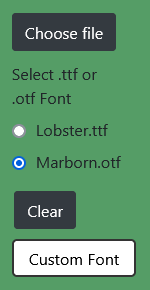
\includegraphics[width=0.3\textwidth]{"images/custom-font.png"}
	\caption{Benutzerdefinierte Fontliste im Texteditor der PDF Web App}
	\label{fig:custom-font}
\end{figure}

Die Fontgröße kann man ebenfalls wie die Zeilenhöhe mit selection menu und input field justieren. Bei der Fontfarbe klickt man auf das initial schwarze Quadrat, was die aktuelle Farbe zeigt, und es öffnet sich ein color picker Menü. Hier kann man die Farbe und Transparenz einstellen. Die Werte kann man sich in RGBA, HSLA oder HEX formatieren lassen. Mit Klick auf die beiden kleinen senkrechten Pfeile im color picker wird jeweils das Format gewechselt. Das Fenster des color pickers für die Fontfarbe ist in Abbildung \ref{fig:fontcolor} abgebildet. 

\begin{figure}[!htbp]
	\centering
	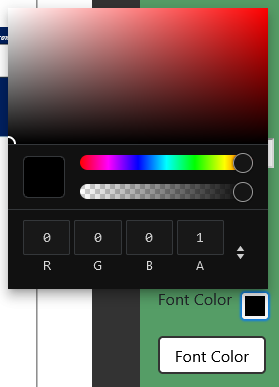
\includegraphics[width=0.5\textwidth]{"images/fontcolor.png"}
	\caption{Color picker für die Fontfarbe des Texteditors der PDF Web App}
	\label{fig:fontcolor}
\end{figure}

Als vorletzte Option kann man den Text absolut drehen. In der Praxis bedeutet das, dass immer eine Benutzereingabe für Rotation das Element mit 0 Grad Rotation auf den gewünschten Wert rotiert. Folglich passiert keine Veränderung, wenn man den gleichen Rotationswert 2 Mal hintereinander ausführt. Abschließend können alle Textelemente im Dokument mit dem Remove Button auf einen Schlag gelöscht werden. Beim Zeilenabstand und der Schriftgröße wird der Benutzer außerdem über den Wertebereich von Benutzereingaben informiert. Man kann generell nur Elemente hinzufügen und auf ihnen die Operationen anwenden. Man kann in der PDF Web App keine im PDF bereits bestehenden Elemente bearbeiten. Die Textoperationen werden in Abbildung \ref{fig:text} demonstriert.

\begin{figure}[!htbp]
	\centering
	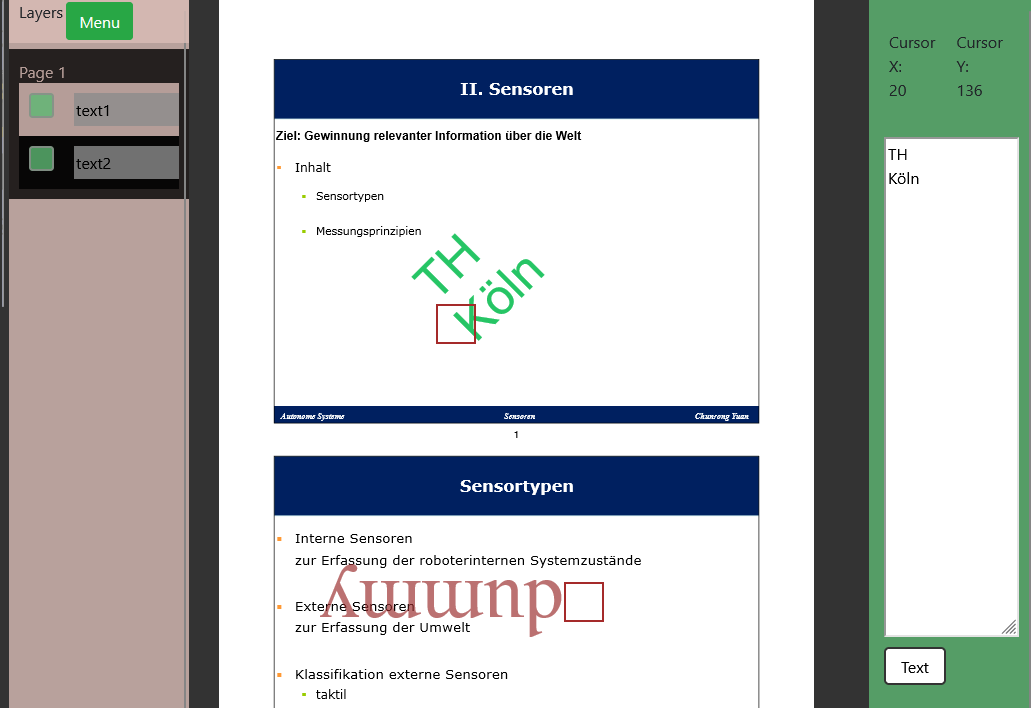
\includegraphics[width=0.9\textwidth]{"images/text.png"}
	\caption{Bearbeiteter Text in der PDF Web App}
	\label{fig:text}
\end{figure}

\subsubsection{Zeichnungen erstellen}
Der Zeichneneditor präsentiert sich einem in Screenshot \ref{fig:drawer}. 

\begin{figure}[!htbp]
	\centering
	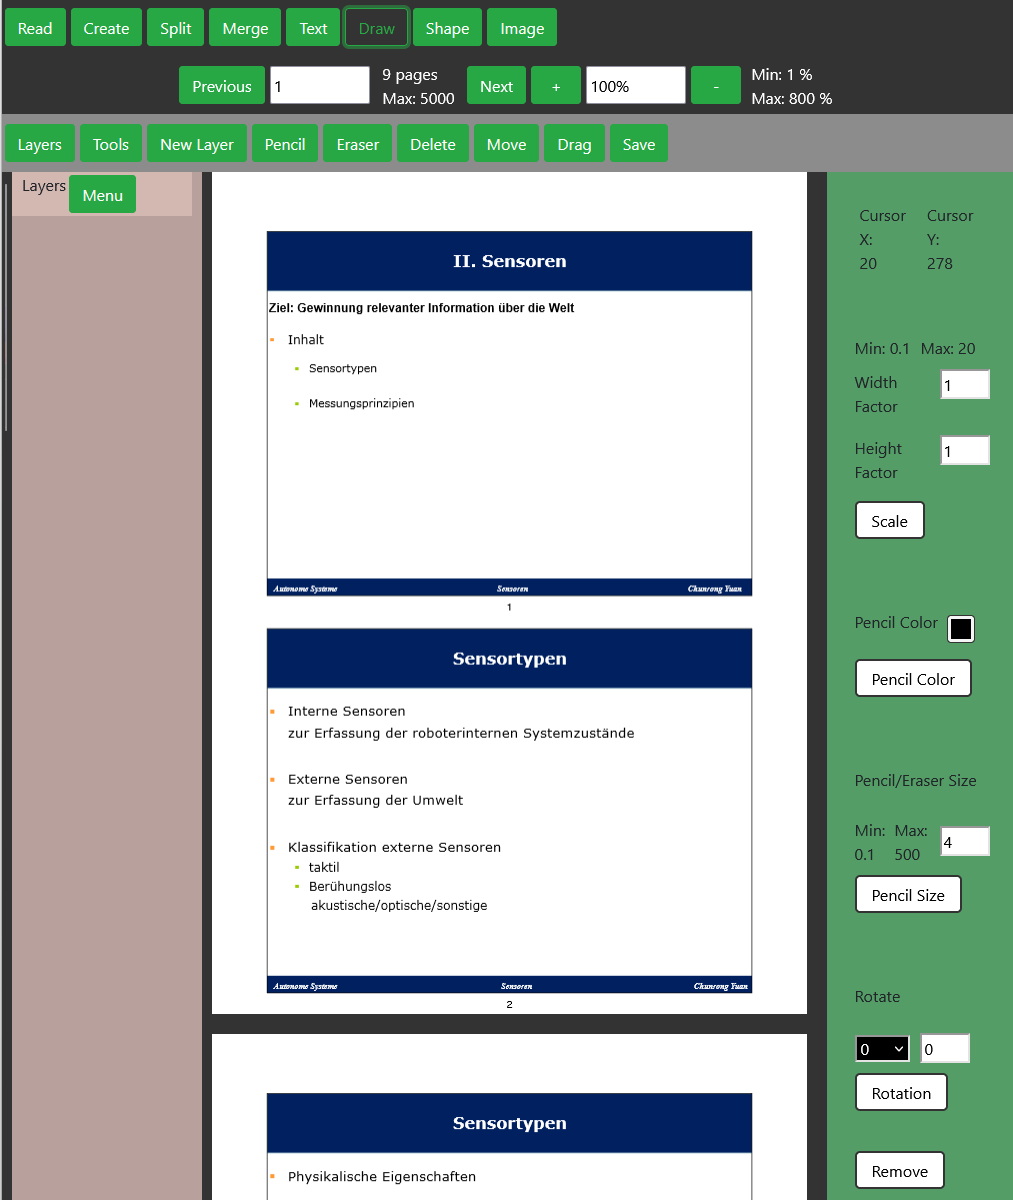
\includegraphics[width=1\textwidth]{"images/drawer.png"}
	\caption{Drawer der PDF Web App}
	\label{fig:drawer}
\end{figure}

Das Ebenenmenü und Tools Seitenmenü des Zeichneneditors erscheint selbst wenn man zuerst im Texteditor ein Dokument geöffnet hat. Nach einem geöffneten PDF kann man von jedem Editor in einen anderen wechseln ohne erneut ein PDF öffnen zu müssen. Mit dem Zeichnen kann man anfangen, wenn man auf Pencil klickt. Bei gedrückter Maustaste auf einer PDF Seite erscheint eine schwarze Linie dort wo die Maus sich bewegt hat. Zusätzlich wird dort wo man angefangen hat die Maus zu drücken eine magenta control box hinzugefügt. Das Zeichnen funktioniert auch mit einem Graphic Tablet. Es wird immer auf der zuletzt gezeichneten Ebene auf der Seite gemalt bzw. wenn man eine Ebene auswählt im linken Ebenenmenü wird auf der ausgewählten Ebene gezeichnet. Ein Klick auf New Layer und anschließender Zeichenmodus mit Pencil kreiert für die neue Zeichnung eine weitere Ebene. Die neue Zeichnung auf der Ebene erhält abermals eine magenta control box. Wurde auf einer Seite bisher noch nichts gezeichnet, so wird bei der ersten Zeichnung auf der Seite eine neue Ebene automatisch angelegt und man muss nicht New Layer drücken. Die Zeichenelemente sind die einzigen Objekte, bei denen der Nutzer selbst die Ebenen einer Seite zuweisen kann mit New Layer. Bei allen anderen Elementen, sei es Text, Geometrie oder Bilder, wird für jedes neue Element automatisch eine Ebene erstellt. Der Radierer ist  mit dem Eraser Button im grauen operations Menü anwendbar. Zuerst drückt man Eraser und geht dann mit gedrückter Maustaste über die Zeichnungen auf einer Seite, die man entfernen möchte. Dort wo bei gedrückter Maustaste die Maus die Linie berührt wird wegradiert. Zeichnen und Radieren bekommen jeweils ein neues Mauscursorsymbol: Beim Zeichnen hat man ein schwarzes dünnes Kreuz und beim Radieren ein weißes dickes Kreuz. Mit dem Delete Button kann man mehrere Zeichnungen nacheinander mit Klicks in die control boxen entfernen. Move und gedrückte Maustaste auf eine control box verschiebt diese. Delete und Move funktionieren analog zum Texteditor. In jedem Editor gibt es einen Delete und Move Button zum Löschen und Verschieben von Elementen. Genau wie alle Operationen im Tools Seitenmenü kann man mit Delete und Move nur die dem Editor zugehörigen Elemente editieren. Im Tools Seitenmenü kann man eine Zeichnung relativ skalieren, indem man einen Faktor eingibt. Der Faktor kann auch ein Float sein und multipliziert sich immer mit der aktuellen Größe, d.h. die aktuelle Größe ist 100 \%. Darunter kann man mit dem color picker menü die Farbe und Transparenz der Stiftfarbe definieren. Sie wird mit einem Klick auf Pencil Color auf die nächste Zeichenoperation angewendet. Außerdem definiert sie auch gleichzeitig die Radiererfarbe, was sich bei Transparenzen unter 1 bemerkbar macht. Sonst ist jede Radiererfarbe gleich, jedoch bei einer Transparenz von unter 1 radiert der Radierer weniger deckend, so als ob man einen Radiergrummi weniger stark auf das Papier drückt. Dann kann man die Größe des Stiftes bzw. Radierers einstellen. Sie greift auch ab der nächsten Zeichen- bzw. Radieroperationen. Ebenfalls kann man Zeichnung mit samt radierten Partien rotieren. Zum Schluss kann man mit Remove alle Zeichnungen im Dokument löschen. Teilweise transparente Zeichnungen werden im Bild \ref{fig:drawing} dargestellt. 

\begin{figure}[!htbp]
	\centering
	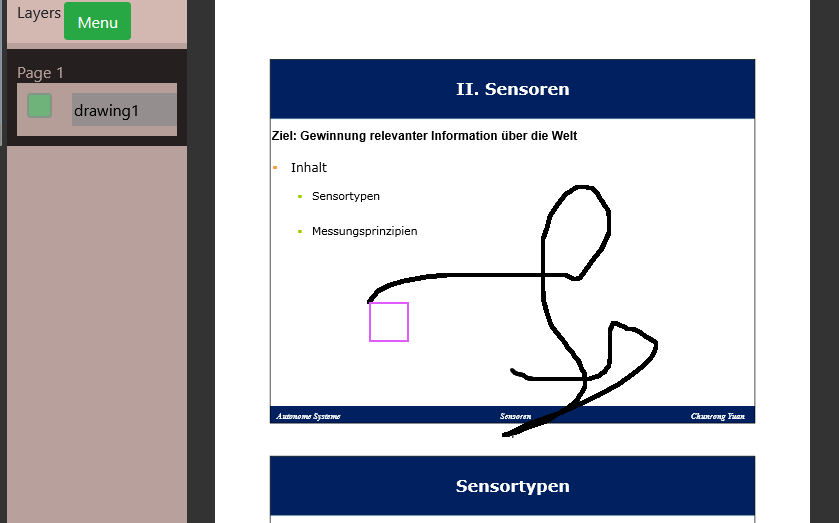
\includegraphics[width=1\textwidth]{"images/drawing.png"}
	\caption{Zeichnungen in der PDF Web App}
	\label{fig:drawing}
\end{figure}


\subsubsection{Geometrie hinzufügen}

\subsubsection{Bilder editieren}

\subsubsection{Arbeiten im Layer Mode}

\subsubsection{Ebenensteuerung}


